\chapter{modified Quadratic Estimator}
\label{ch:analysis}
\section*{Overview}\label{ovr}
In this chapter we discuss modified Quadratic Estimator which we have developed to eliminate the bias due thermal Sunyaev Zel'dovich (SZ) effect. 
We give a brief review thermal Sunayev-Zel'dovich effect (refer \pending{citations} for a detailed review)and its effect on cluster lensing in the \S\ref{tsz}.
Then we discuss the modifications of the QE to remove SZ bias in \S\ref{sec_method}.
 Later we explain the SPTpol and DES data sets in \S\ref{sec_data}, results in \S\ref{sec_results} and quantify systematics in \S\ref{sec_systematics}.
Finally we conclude in \S\ref{sec_conclusions}.
%We explain the constraints on mass-richness scaling relation obtained using the above data. 


\section{Thermal Sunayev-Zel'dovich effect}\label{tsz}

 Cosmic microwave background (CMB) photons gets inverse Thompson scattered off the high energetic electrons present in the intra cluster medium of a galaxy cluster, resulting in a deficiency of photons at lower frequency and excess of photons at higher frequency. 
 This phenomena is called thermal Sunayev-Zel'dovich effect (SZ). 
 SZ is a small effect and to illustrate it we have shown CMB spectral distortion for a fictional galaxy cluster of mass 1000 times more that of a typical galaxy cluster in Fig ~\ref{ned_plot}.
 The solid black curve represents the intensity of CMB as a function of frequency before its interaction with hot intracluster medium; solid blue represents the same after its interaction.
 As shown in the Fig.~\ref{ned_plot}, SZ decreases the intensity of CMB below a frequency of ~ 220 \,GHz and increases at higher frequencies. 
   
The fractional change in temperature is given by 
\begin{equation}
\label{eq:sz_eqn}
\frac{\Delta T_{SZ}}{T_{CMB}} = f(x) y = f(x) \int n_{e} \frac{k_{B}T_{e}}{m_{e}c^{2}} \sigma_{T} dl
\end{equation}
where $y$ is Compton $y$-parameter, $n_{e}$ is the electron number density, $m_{e}$ is the electron rest mass, $c$ is the speed of light,  $T_{e}$ is the electron temperature, $\sigma_{T}$ is the Thompson cross-section, and f(x) is the dimensionless frequency given by
\begin{equation}
f(x) = (x\frac{e^{x}+1}{e^{x}-1} -4)(1 + \delta_{SZE}(x,T_{e}))
\end{equation} 
where $\delta_{SZE}(x,T_{e})$ is the relativistic correction to the frequency dependence.
\begin{figure}
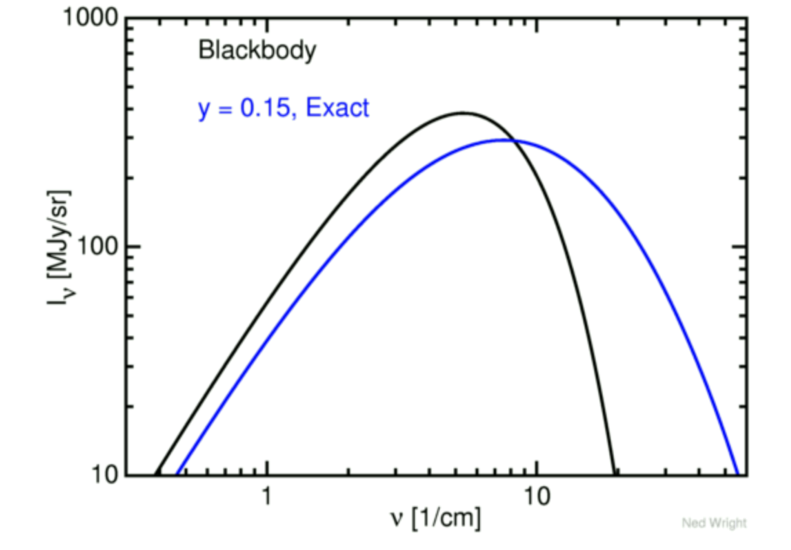
\includegraphics[width=\linewidth]{figs/tSZ_effect_Ned.png}
\label{ned_plot}
\caption{The plot shows the intensity of CMB as function of frequency before (black) and after (blue) it passes through a cluster. }
\end{figure}

As can be seen in \ref{eq:sz_eqn} SZ effect is independent of redshift and has potential to high redshift clusters, where the cluster abundance critically depends on underlying Cosmology.
CMB surveys use SZ effect to detect galaxy clusters; %, galaxy clusters appears as blue blob at frequencies lesser than 220 \, GHz.
Fig. \ref{fig:clus_in_cmb} shows a galaxy cluster of mass $M_{200m}\footnote{$M_{200m}$ is defined as the mass of the cluster within a radius $R_{200}$, within which the cluster density is 200 times the critical density of the Universe at cluster redshift} = 5*10^{14} M_{\odot}$ as seen by CMB survey in 90\, GHz and 150\, GHz channels . 
\begin{figure}
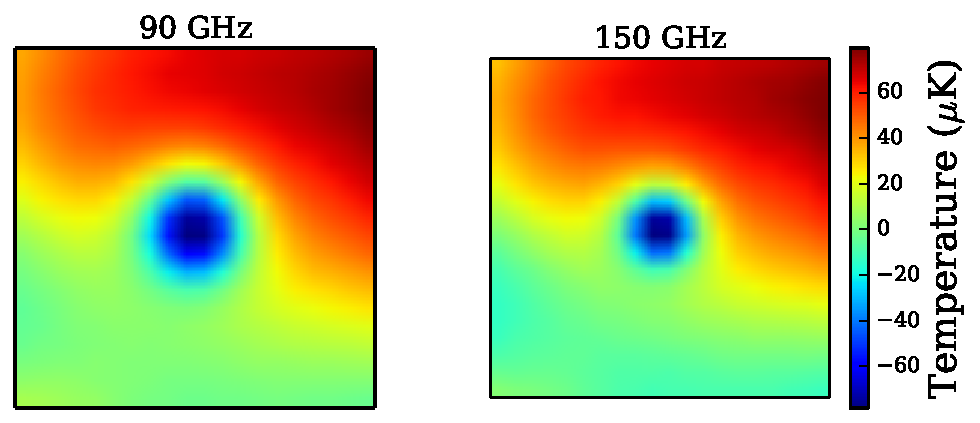
\includegraphics[width=\linewidth]{figs/clus_in_cmb}
\label{fig:clus_in_cmb}
\caption{Galaxy cluster of mass $M_{200m} = 5*10^{14} M_{\odot}$ as seen in a CMB survey with following specifications : 1.\arcmin7  beam at 90 \,GHz (left panel) and 1\arcmin  beam at 150 \, GHz (right panel). }
\end{figure}
 
 Though SZ is small spectral effect, it is still much higher than the lensing signal. 
 It is an order of magnitude greater than the lensing signal and hence induces a significant systematic and statistical uncertainty if not taken into account. 
 Fig ~\ref{fig:SZ_effect} shows the effect of SZ on the lensing convergence profile. 
 In the left panel of figure we show the stacked lensing convergence profile of 1000 clusters each with a mass of $4*10^{14}$ $M_{\odot}$ and an experimental noise of 1\ukam with no SZ and on the right panel is with the SZ.  
 As can be inferred from the plot, presence of SZ induces a blue blob in the center and hence resulting in a negative bias.
 \begin{figure}
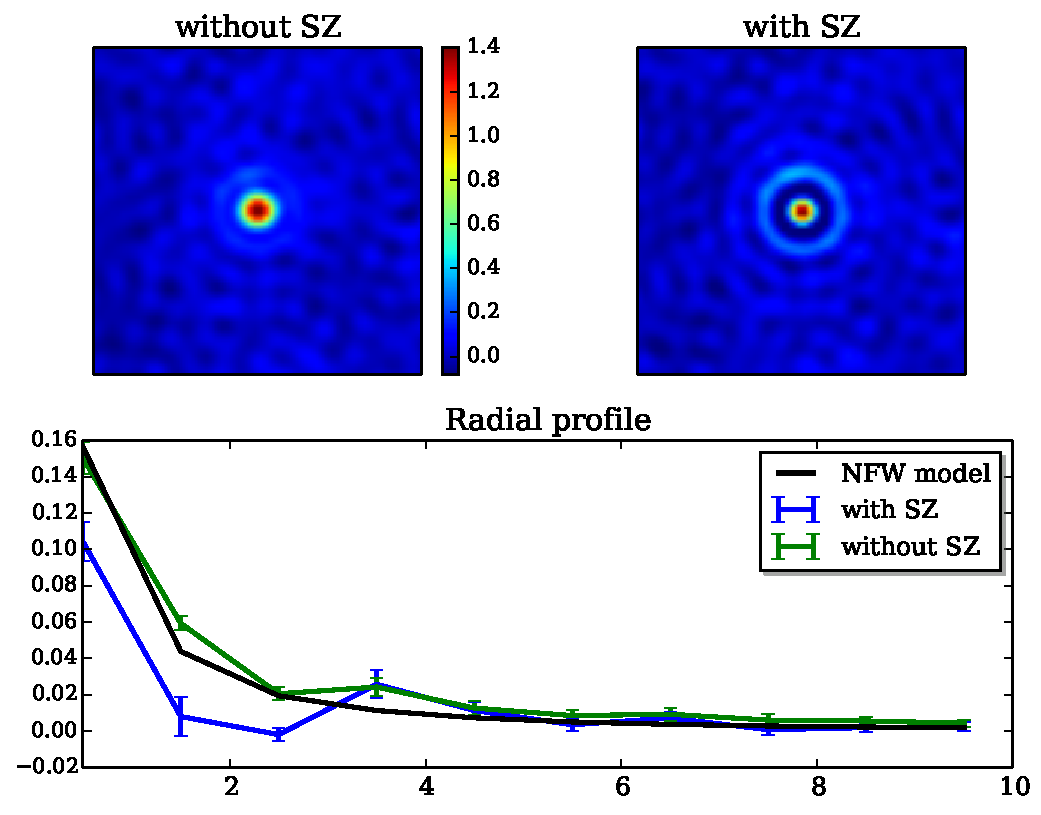
\includegraphics[width=\linewidth]{figs/tSZ_effect_on_lensing.pdf}
\caption{Effect of SZ on lensing convergence profile. On the top panel we show the lensing convergence profile for a stack of 1000 cluster each at a mass of $M_{200m}= 2*10^{14}  M_{\odot}$ and a redshift of $z = 0.7$ with experimental white noise level of $3\ukarcmin$; left panel is without SZ and right panel is with SZ. On the bottom panel we have radial profile of the same in solid blue (without SZ) and green (with SZ) curves; black curve is the radial profile of the input NFW profile. }
\label{fig:SZ_effect}
\end{figure}



\section{Methods}
\label{sec_method}
\subsection{Quadratic Estimator}
%Quadratic Estimator is based on two approximations: gradient approximation and linearization in convergence.

Typical size of galaxy cluster is of the order of few arc minutes. 
Primordial CMB doesn't have power at such small scales due to diffusion damping \cite{Silk} and can be approximated as a gradient. 
Lensing due to galaxy cluster induces a dipole kind of structure oriented along the direction of background gradient with hot and cold spots swapped.
For a given cluster mass and redshift, the magnitude of this dipole scales linearly with the magnitude of the CMB gradient.
This correlation between the unlensed CMB gradient and lensing signal is known as the gradient approximation and is equivalent to
\begin{equation}
T (\hat{n})\approx \tilde{T}+ \nabla T . \vec{\alpha}(\hat{\textbf{n}})
\end{equation}
Below we provide the mathematical formalism for temperature quadratic estimator and it generalises for polarisation.

 Under the gradient approximation, we construct an estimator of lensing convergence by multiplying the lensing map and the gradient map.
The gradient approximation doesn't hold for all Fourier modes, only for the modes which are correlated by reconstruction.
We filter maps in the Fourier space to isolate modes for which the gradient approximation is valid.
%\begin{equation}
% \hat{k_{l}} = -A_{l} \int d^{2} \hat{n} e^{i\hat{n}.l} Re{\nabla .[G(\hat{n}) L^{*}(\hat{n})]}
 %\end{equation}
 We obtain gradient and lensing maps as follows,
 % $G(\hat{n})$, $L(\hat{n})$ are filtered gradient and lensing maps respectively, $A_{l}$ is the normalisation parameter.
 % We obtain $G(\hat{n})$, $L(\hat{n})$ from the observed temperature map as follows
  \begin{eqnarray}
  L(\hat{n}) = \int \frac{d^{2}l}{(2\pi)^{2}} e^{il .\hat{n}} W^{T}_{l} T_{l}\\
  G(\hat{n}) = \nabla (\int\frac{d^{2}l}{(2\pi)^{2}} e^{il .\hat{n}} W^{TT}_{l} T_{l}   )
  \end{eqnarray}
  where $G(\hat{n})$, $L(\hat{n})$ are filtered gradient and lensing maps and $T_{l}$ is the observed temperature map in Fourier space.  
 Fourier filters $W^{T}_{l}$ and $W^{TT}_{l}$ are given by 
 \begin{eqnarray}
 W^{T}_{l} = (C^{TT}_{l} + N^{TT}_{l})^{-1}\\
 W^{TT}_{l} =  \widetilde{C}^{TT}_{l}(C^{TT}_{l} + N^{TT}_{l})^{-1}
 \end{eqnarray}
 where  $\widetilde{C}^{TT}_{l}$,$C^{TT}_{l} $  is the unlensed and large scale structure lensed CMB power spectrum obtained from \texttt{CAMB}, $ N^{TT}_{l}$ is the experimental noise power spectrum.
 With filtered gradient and lensing maps in hand we can write down the expression for lensing convergence profile as 
 \begin{equation}
 \hat{k_{l}} = -A_{l} \int d^{2} \hat{n} e^{i\hat{n}.l} Re{\nabla .[G(\hat{n}) L^{*}(\hat{n})]}
 \end{equation}
 where $A_{l}$ is the normalisation parameter given by
 \begin{equation}
 \frac{1}{A_{l}} = \frac{2}{l^{2}} \int \frac{d^{2}l_{1}}{4\pi^{2}} (l.l_{1}) W^{TT}_{l} W^{T}_{l} (\tilde{C}^{TT}_{l_{1}}(l.l_{1}) + \tilde{C}^{TT}_{l_{2}}(l.l_{2}))
 \end{equation}
 where $l = l_{1}  + l_{2}$. 
  \subsection{mitigating magnification bias}
Galaxy cluster magnifies the background image and decreases the observed temperature gradient behind it, which leads to a low bias in lensing reconstruction.
The bias is due to the overlap in scales between the unlensed temperature gradient and the lensed temperature field. 
Though wiener filter reduces the bias, it is not removed completely.
We can reduce the bias further by exploiting the prior knowledge on unlensed CMB power spectrum.
 From Fig.~\ref{fig:gradient_cut}, which shows the unlensed rms gradient as a function of multipoles, it is evident that most of the power for the gradient map comes from scales below $l$<2000.
 By low pass filtering the gradient map, we separate the unlensed temperature gradient and the lensed temperature field with almost no loss in SNR.
 \begin{figure}
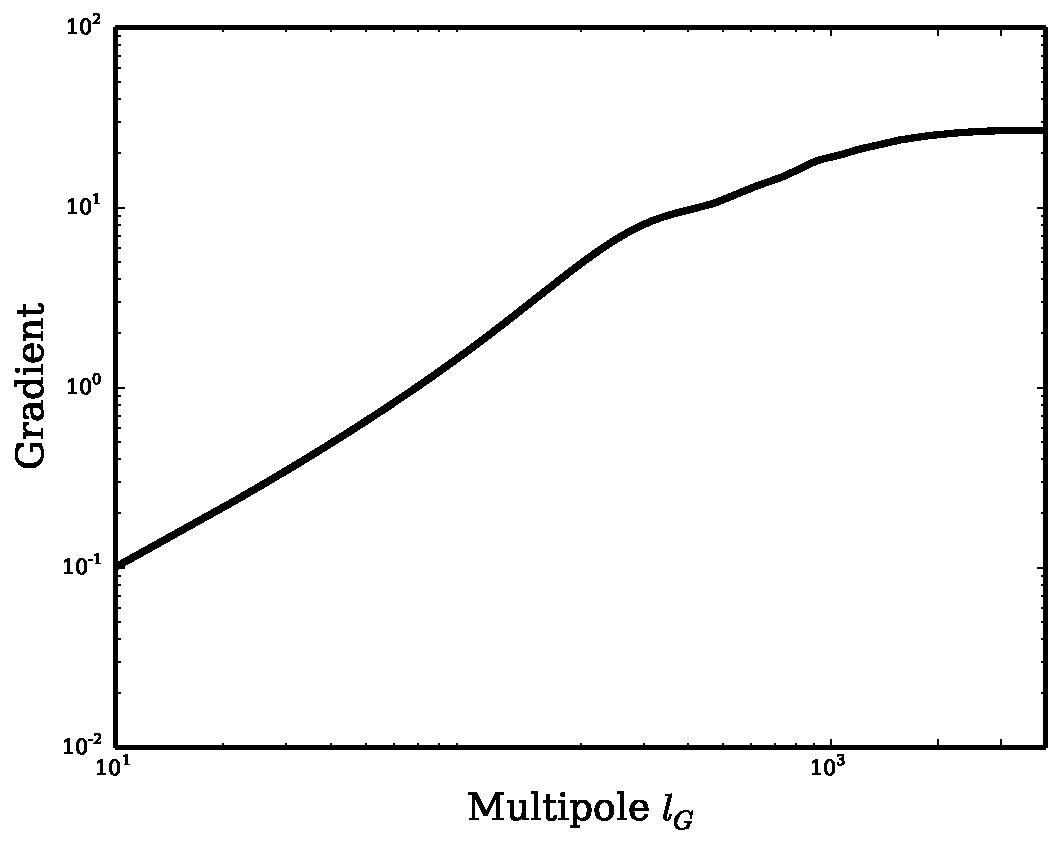
\includegraphics[width=\linewidth]{figs/gradient_cut.pdf}
\caption{Gradient of temperature field as a function of low pass filter l = $l_{G}$. It is dominated by mulitpoles below 2000. \pending{check the magnitude, remake the plot}}
\label{fig:gradient_cut}
\end{figure}
The schematic representation of Quadratic Estimator is shown in Fig 2. 
Panel (a) is the 10\arcmin X 10\arcmin cutout of the observed temperature map, $T_{l}$.
This is filtered in the fourier space \pending{mention equations} to obtain the filtered gradient and lensing maps, shown in panel (b) and (c) respectively.
Lensing convergence profile (panel (c)) is reconstructed by extracting the correlations between lensing and gradient maps.
 \begin{figure}[H]
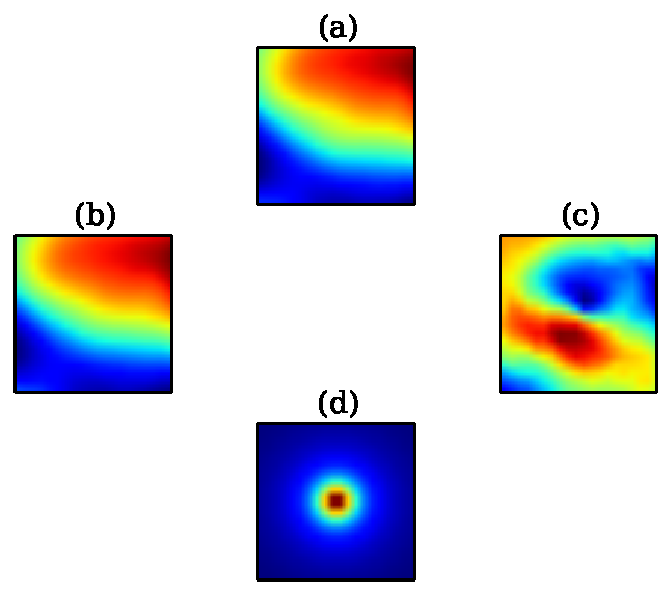
\includegraphics[width=\linewidth]{figs/QE_schem.pdf}
\caption{Schematic representation of Quadratic Estimator. Top panel shows the observed CMB temperature map which acts as the input, which is passed through the filters to obtain large scale gradient map (panel 'b') and small scale lensing map (panel 'c'). QE extracts the correlation between panel 'b' and 'c ' to obtain reconstructed lensing convergence profile shown in panel 'd'}
\label{fig:QE_schem}
\end{figure}
 
\section{modifications of Quadratic Estimator}
The major foreground in CMB cluster lensing analysis is SZ effect.
SZ effect is an order of magnitude greater than lensing signal; if not taken into consideration it induces systematic bias and variance in the final convergence maps.
In this section we describe the modifications of Quadratic Estimator which eliminates the SZ induced bias, in the next chapter we discuss the method to reduce SZ induced variance.


\subsection{modified Quadratic Estimator}
While designed to pull the lensing induced correlations, QE is equally sensitive to any other signal present in both G and L maps.
%The major systematic for lensing analysis is thermal Sunyaey -Zel'dovich (tSZ) effect, which is an order of magnitude greater than lensing signal biases the analysis if not taken into account. 
 SZ present in both maps results in a low bias if not taken into account \ref{fig:SZ_effect}.
 Two methods have been discussed in literature to eliminated/mitigate the SZ bias:
 one way to eliminate SZ bias is by using SZ free maps, which are constructed by exploiting the spectral dependance of SZ signal.
 %Previous studies either used a tSZ free map or a more stringent low pass filtering of the gradient map.
 %tSZ is frequency dependent signal and hence we can use multiple frequency channels to eliminate tSZ. 
 However, this results in an increased statistical uncertainty in the reconstructed convergence profile.
 Another way to mitigate the bias is by using a more stringent low pass filter on the gradient map, having a robust separation of scales between gradient map and small scale map reduces SZ correlation.
 While this can reduce the bias significantly,  poor gradient estimation results in an increased statistical uncertainty.

 
 During my thesis we came up with a novel approach to completely remove the SZ bias. 
 Any foreground signal which is present in both the maps will lead to a systematic bias, so by getting rid of the foreground signal in one of the maps (either G or L) should eliminate the bias completely.
  As shown in Fig.~\ref{fig:gradient_cut}, most of the gradient estimation comes from multipoles $l$ <2000 where CMB is not limited by experimental noise.
  So, natural choice would be to eliminate SZ in the gradient map by using linear combination of different frequencies. 
  In modified Quadratic Estimator, eqn 3.6 becomes,
  \begin{equation}
   G(\hat{n}) = \nabla (\int\frac{d^{2}l}{(2\pi)^{2}} e^{il .\hat{n}} W^{TT}_{l} T^{SZ_free}_{l}   )
  \end{equation}
  where $T^{SZ free}_{l} $ is an SZ-free map.
\section{Data}
\label{sec_data}
We use data sets from two different experiments: CMB maps from South Pole Telescope is explained in \S\ref{sec_SPT} and 
optical cluster catalog from Dark Energy Survey is explained in \S\ref{sec_DES}

\section{South Pole Telescope}
\label{sec_SPT}
South Pole Telescope (SPT) is a 10 meter diameter, wide field, offset Gregorian telescope \citep[SPT,][]{padin08, carlstrom11} located at the Amundsen-Scott South Pole station.
The SPT has been operating since early 2007 and has completed two surveys so far: SPT-SZ (2007 -2011) and SPTpol (2012-2016).  
Extremely dry and stable atmosphere of the south pole makes it one of the best available sites on Earth for observing millimeter and sub-millimeter wavelengths. 

\subsection{\sptpol{} {\rm 500} deg$^{2}$ survey}\label{sec_sptpol}
\sptpol{} is the second camera installed on the \mbox{10-meter} South Pole Telescope \citep[SPT,][]{padin08, carlstrom11}.
The \sptpol{} focal plane consists of 1536 polarization-sensitive transition edge sensor bolometers (360 at 95 GHz and 1176 at 150 GHz) \citep{austermann12}.
%enabling polarization observations \citep{austermann12}.
The \sptpol{} 500~deg$^{2}$ survey spans fifteen degrees of declination, from -65 to -50 degrees, and four hours of right ascension, from 22h to 2h. 
%In this work we use the temperature (T) and polarization (Stokes Q and U) maps of the CMB from observations between April 2013 to September 2016 in the frequency bands 95 GHz and 150 GHz. 
In this work, we use CMB temperature maps from observations between April 2013 and September 2016 in frequency bands centered at approximately 95 GHz and 150 GHz. 
\pending{include scanning strategies}
The telescope beam and pointing solutions were characterized using Venus and bright point sources in the \sptpol{} survey region. 
The final telescope beam along with the pointing jitter roughly corresponds to a $\theta_{\rm FWHM} = 1.^{\prime}22\ (1.^{\prime}7)$ Gaussian for the 150 (95) GHz dataset.

We briefly summarize the procedure we use to reduce raw CMB data to maps and refer the reader to \cite{henning18} for further details. 
The raw data are composed of digitized time-ordered data (TOD) for each detector that are converted into CMB temperature units. %% using a Planck-based calibration factor. 
We bin the TOD into two different maps using a flat-sky approximation in the Sanson-Flamsteed projection \citep{calabretta02, schaffer11}. 
To construct the first map, in which we aim to reconstruct the small-scale lensing signal, we remove large-scale modes $\ell \le 300$, bandpass filter the TOD in the range of approximately $300 \le \ell_{x} \le 20,000$, and bin them into 0.\am5\ square pixels.
For the second map, intended for estimation of the large-scale CMB gradient, we apply minimal TOD filtering by only removing modes below $\ell_{x} \le 30$, and bin them into 3\am\ square pixels.
While we only use the data from the 150 GHz channel for the first map, the latter is a tSZ signal cleaned map produced by linearly combining the 95 and 150 GHz channels. 
We use this tSZ-free map to reconstruct the background gradient of the CMB at the cluster locations.
As we will see later in \S\ref{sec_method_QE}, the gradient estimation using the tSZ-free map helps in removing the tSZ-induced lensing bias.
The minimal filtering on this map allows us to recover large-scale modes which indeed helps in a better estimation of the background gradient.
The 0.\am5{} resolution 150 GHz map has a white noise level of \mbox{$\Delta_{\rm T} = $ 6 \ukam} estimated using a jackknife approach. %estimated within the multipole band $4500 \le \ell \le 7500$.
The low-resolution tSZ-free combination is noisier with \mbox{$\Delta_{\rm T} \sim $ 17 \ukam}.
\pending{Noise power spectrum plot}
%%%\pending{Pending: SR: Should we quote this? Can we trust this number?}
%\section*{Cosmic Microwave Background cluster lensing}
\subsection{DES and the {\rm \RM} catalog}\label{sec_DES}
The Dark Energy Survey (DES) was a $\sim$5000 \sqdeg, optical to near-infrared survey conducted using the Dark Energy Camera \citep{flaugher15} mounted on the 4-meter Victor Blanco telescope at Cerro Tololo Observatory in Chile and has recently finished its survey. 
For this analysis, we use the cluster catalog obtained from the first three years of DES observations, which almost covers the \sptpol{} 500\,deg$^{2}$ survey. 

%The cluster catalog was derived using the RM algorithm \citep{rykoff14}  from the DES photometric datasets. 
The cluster catalog was derived using the RM algorithm \citep{rykoff14}.
RM is an optical cluster-finding algorithm which detects candidates by identifying over-densities of luminous red galaxies with luminosity greater than 20\% of $L_{*}.$
%Milky Way ($0.2L_{*}$). [I DON'T THINK THIS IS ACTUALLY THE DEFINITION OF L* (TC\citetalias{mcclintock18})]
It is based on our understanding that galaxy clusters are agglomerations of galaxies containing old and subsequently red stars. 
The algorithm iteratively assigns membership and centering probabilities for each red galaxy identified as belonging to a cluster candidate. 
A weighted sum of the membership probabilities, richness $\lambda$, is assigned to each candidate.
The centre comes from the galaxy with the highest centering probability.
The DES RM catalog contains two samples: a flux-limited sample and a volume-limited sample. 
The flux-limited sample has more high-redshift clusters detected from deep fields in the survey. 
On the other hand, the volume-limited sample is independent of survey depth, complete above a luminosity threshold \citep[hereafter \citetalias{mcclintock18}]{mcclintock18}, and normally preferred for cosmological analysis.
% (hereafter referred to as the volume-limited sample).
See \citet{rykoff16} for more information on the application of RM to the DES survey data.

The RM cluster catalog version employed in this analysis is \whichcatversion. 
The \whichyear{} gold catalogue is based on the previous catalog from the Year-1 data \citep{drlica-wagner17} with some updates described in \citet{morganson18}.
The catalog contains 54,112 clusters above richness $\lambda \ge 20$ in the flux-limited sample and 21,094 clusters in the volume-limited sample. % \pending{(Pending: Cite DES Y3 cat. paper)}. 
Of these, 5,828 (2,428) clusters from the flux(volume)-limited sample lie within the \sptpol{} 500 \sqdeg{} survey  in the redshift range $0.1 \le z \le$ 0.95 (0.90). 
%We additionally remove clusters near the survey edges or within $10^{\prime}$ distance from a bright ($\ge 50$ mJy at 150\,GHz) point source.
We additionally remove clusters near the survey edges by removing the cutouts (see \ref{sec_cluster_cutouts}) with more than 5\% masked pixels or within $10^{\prime}$ distance from any bright ($\ge 6$ mJy at 150\,GHz) point sources detected in the \sptpol{} temperature map.
%we use data/500sqdeg_bleem/quick_mm_point_source_file_150.0GHz_6.00000mJy.txt.
These cuts leave 4,003 (1,741) clusters with $\lambda \ge 20$ from the flux(volume)-limited sample with a median redshift of $\tilde{z}$ = 0.77 (0.48). 
The error in the cluster photo-$z$ estimates are small with $\hat{\sigma}_{z} = 0.01 (1+z)$ \citep{rozo15}.
\pending{include a SPTpol map pointing to a cluster}
%\pending{Finally, we impose a cut on the cluster richness and remove all clusters above $\lambda \ge 60$ that removes \pending{xx (xx)} from the full (cosmology) sample. This cut was motivated based on the results from Sehgal sims described in \S\ref{sec_xx_xx}}.
%Cosmic Microwave Background (CMB) photons while passiang through intervening galaxy cluster gets lensed and we call this phenomenon as CMB-cluster lensing.
% Lensing remaps the unlensed CMB field based on the angular deflection caused by cluster gravitational potential.
 %In mathematical form CMB cluster lensing can be written as the equation below
 %\begin{eqnarray}
%T(\hat{\textbf{n}})& = & \widetilde{T} (\hat{\textbf{n}} + \vec{\alpha}(\hat{\textbf{n}}))\\
%Q(\hat{\textbf{n}}) & = & \widetilde{Q} (\hat{\textbf{n}} + \vec{\alpha}(\hat{\textbf{n}}))\\
%U(\hat{\textbf{n}}) & = & \widetilde{U} (\hat{\textbf{n}} + \vec{\alpha}(\hat{\textbf{n}}))
%\end{eqnarray}
%where $ \widetilde{T}$ is unlensed temperature field, $\widetilde{U}$ and $\widetilde{Q}$ are the unlensed polarisation fields.
%$\vec{\alpha}(\hat{\textbf{n}})$ denotes the deflection angle and is directly proportional to the mass of the galaxy cluster.

%Lensing signal by an individual cluster is too weak to detect, so we need to stack many clusters to obtain a significant signal.
 %For example, the lensing induced distortion due to a $2 \times 10^{14} \ M_{\odot}$ mass galaxy cluster  is $\sim 5.0$ and $0.5 \ \mu K$ in temperature and polarization respectively.
%In this chapter, we will discuss various methods available in literature to extract CMB-cluster lensing signal. 
%The chapter is organized as follows 
 \section{cluster cutouts and model fitting}
 
 In this section first we describe the extraction of cluster cutouts from SPTpol maps in \ref{sec:cluster_cutouts}, followed by model fitting in \ref{sec:model_fitting}. 
 
 
 \subsection{Cluster cutouts}
 \label{sec:cluster_cutouts}
 We extract 300\arcmin square box form SPTpol temperature maps at the DES cluster locations. 
While the boxsize is much larger than the virial radius of the cluster, it is necessary to robustly approximate the background gradient. 
This is because much of the gradient power comes from larger scale modes, reducing the analysis to a smaller box will reduce the SNR of the mass estimation. 
These cutouts are then passed through the pipeline to extract lensing convergence profile, after which we limit the modelling and likelihood calculations to 10\arcmin box around a cluster to lessen the computational effort.

As mentioned before, the lensing signal is weak for individual cluster and we need to stack lensing convergence profiles to increase the SNR of detection.
 Thus the stacked convergence map is simply: 
 \begin{equation}
 \hat{\kappa} = \frac{\sum_j  w_j \left[ \hat{\kappa}_{j} - \left< \hat{\kappa}_{j} \right> \right]}{\sum_j w_j} - \hat{\kappa}_{\rm MF},
 \end{equation}
% where the subscript $j$ refers to an individual cluster and the weighting scheme $w$ is described below.
 where $\hat{\kappa}_{j}$ refers to reconstructed convergence map of cluster $j$ %satisfying $\left< \hat{\kappa}{\rm C}_{j} \right> = 0$ 
 and the weighting scheme $w$ is described below.
From the stacked map, we remove all modes above the \sptpol{} 150 GHz beam scale of $\theta_{\rm FWHM}\sim 1.^{\prime}2$. 
%Relaxing this filter does not contribute much to the \snr{} as those modes are either dominated by foregrounds or noise. 
We also remove an estimate of the mean-field $\hat{\kappa}_{\rm MF}$ from this stacked convergence map.
The mean-field arises because of two reasons.
One because the temperature maps, before being filtered using Eq. (\ref{eq_QE_filtered_gradient_lensing_maps}), are apodized using a Hanning window with a $10^{\prime}$ edge taper to reduce edge effects.
The other reason is the presence of inhomogeneous noise in the survey region.
We obtain the mean field bias by stacking the convergence maps reconstructed at \howmanyrandomsforMF{} random locations in the maps. 


{\it Weighting scheme:} We decompose the weights for each cluster into two components: 
The first is the inverse-noise-variance weight, $w_{k}$, constructed from the observed standard deviation $\sigma_{\kappa}$ in the reconstructed \sptpol{} convergence maps in a ring between $10^{\prime}$ and $30^{\prime}$ around the cluster. 
The noise in convergence is proportional to the noise in the associated gradient map and increases, as expected, when $\ell_{\rm G}$ is reduced.
The second\footnote{We note that for the mean-field reconstructed from random locations, we only apply the weight $w = 1/\sigma_{\kappa}^2$ for stacking.} weight comes from the noise in the convergence maps due to the presence of SZ signal in the second leg of the QE, the \sptpol{} 150 GHz map.
While our method completely eliminates the SZ-induced lensing bias, the presence of SZ signal in the second map tends to increase the variance in the convergence maps. 
The noise is proportional to the SZ brightness and, as expected, is higher for massive clusters.
For example, the lensing signal of a cluster is proportional to its mass $M$ while the SZ signal scales roughly as $M^{5/3}$.
%Given that our cluster sample contains $\le 4\%$ clusters with richness $\lambda \ge 60$ (\mbox{\mvir\ $\sim 5.2\ \times$ \munits} at $z=0.5$), this extra noise does not completely average out and our results are sample variance limited.


We obtain this second set of weights, $w_{\rm SZ}$, using simulations. 
For every cluster in the DES sample, we reconstruct the convergence profile using a simulated SZ-free gradient map and a 150 GHz map with SZ signal assuming an Arnaud profile \citep{arnaud10} with a log-normal scatter of 20\% in the $Y_{SZ}-M$ relation. 
We turn off cluster lensing, as the objective here is to only get an estimate of the SZ-induced noise in the convergence maps.
%A total of 25 simulations were used to get the noise estimate for each DES cluster and we perform two sets of simulations: one with \sptpol{} tSZ-free gradient map and the other with \lgmca{}.
A total of 25 simulations were used to get the noise estimate for each DES cluster.
The weights are estimated as
%using the inverse noise variance 
$w_{\rm SZ} = 1/\sigma_{\rm SZ}^{2}$, where $\sigma_{\rm SZ}$ is the standard deviation of the `null' convergence map within an angular distance of $10^{\prime}$ from the cluster centre.
%The errors increase with richness and take a power law form parameterized as $\sigma_{\rm SZ}(\lambda) =  \sigma_{0}\lambda^{\alpha}$ with values $(\sigma_{0}, \alpha) = (0.0045, 1.55)$ for the \sptpol{} $\times$ 150 GHz and $(\sigma_{0}, \alpha) = (0.0066, 1.39)$ for the \lgmca{} $\times$ 150 GHz cases. \pending{(Pending SR: I must think a bit more if it makes sense that the weights change when the gradient map (/noise) changes.)}
The errors increase with richness and take a power law form parameterized as $\sigma_{\rm SZ}(\lambda) =  \sigma_{0}\lambda^{\alpha}$ with values $%%%commentingthisoutfornow(\sigma_{0}, \alpha) = \pending{(0.0045, 1.55)}$.
(\sigma_{0}, \alpha) = (0.0045, 1.55)$.
The results are unchanged if we derive the weights using the SZ signal from \citetalias{sehgal10}.
%The standard deviations vary by up to a factor of \pending{six}, based on the local survey noise and point source mask, although 90\% of the standard deviations are within a factor of \pending{two} of each other. 
 % We choose to use uniform weights across the N-cluster sample, $w_j = 1/N$. 
The total weight is now:
 \begin{equation}
 w = \frac{1}{\sigma_{\kappa}^{2} + \sigma_{\rm SZ}^{2}}.
\label{eq_cluster_weight}
 \end{equation}

Introducing $w_{\rm SZ}$ down-weights the most massive clusters, reducing the contribution
of clusters with $\lambda \ge 60$ to less than 1\% in the final stacked sample. 
This is why the change in gradient-map LPF scale to \mbox{$\ell_{\rm G} = 1000$} from the fiducial \mbox{$\ell_{\rm G} = 2000$}
for these clusters (see \S\ref{subsec_QE_modificaltion}) has negligible effects in our final results. 

An alternative to this down-weighting is to swap the maps in the two legs of the QE (i.e. the 150 GHz map for the gradient estimation and the tSZ-free map to reconstruct lensing) for clusters with \mbox{$\sigma_{\rm SZ} > \sigma_{\kappa}$}, which is approximately true for clusters with $\lambda > 40$. However, this results in a minimal gain as the \sptpol{} SZ-free map has a higher noise ($\times3$) compared to the \sptpol{} 150 GHz maps. 
In the next chapter, we discuss the template fitting approach used to reduce the SZ variance significantly.
%Some other approaches to handle the additional noise from the tSZ signal include (a) rotating the reconstructed lensing map based on the direction of the background CMB gradient and fitting for the tSZ-noise, (b) removing a matched-filter estimate of the tSZ-signal from the 150 GHz map before passing the map into the QE. We will explore such possibilities in detail in a future work (Patil S. et al. 2019, in preparation).
 \subsection{Model Fitting}
 \label{sec:model_fitting}
To obtain the mass of the cluster, we need to compare the observed lensing profile to the convergence model generated using an assumed halo mass profile.
 The observed lensing convergence profile of cluster has contributions from its own halo density ($k_{1h}$) as well as from the correlated structures along the line of sight known as two halo term ($k_{2h}$).
 For $k_{1h}$, we assume the galaxy cluster density to follow Navarro Frenk White (NFW) profile and in \ref{sec_systematics} we quantify the robustness of this assumption by using Einasto profile \citep{Einasto}.
 A NFW halo profile is characterized by its scale radius $R_{s}$, the dimensionless concentration parameter c, and the dimensionless charateristic over-density $\delta_{c}$.
 The characteristic over density is defined as the ratio of central cluster density to the critical density of the Universe at the cluster redshift.
 In terms of these quantities the NFW halo density profile is written as 
 \begin{equation}
 \rho(r) = \frac{\delta_{c}\rho_{crit,z}}{(\frac{r}{R_{s}})(1 + \frac{r}{R_{s}})^{2}}
 \end{equation} 
 where $\rho_{crit,z}$ is the critical density of the Universe at cluster redshift.
 
 The lensing convergence profile is the ratio of surface mass density to the critical surface density of the Universe at cluster redshift, $k(x) = \frac{\Sigma(x)}{\Sigma_{crit}}$, where
 \begin{eqnarray}
 \Sigma(x) = 2 \int^{\inf}_{0} \rho(r) ds\\
 \Sigma(crit) = \frac{c^{2}}{4\pi G} \frac{D_{CMB}}{D_{clus} D_{CMB,clus}} 
 \end{eqnarray} 
Here r is the distance from the center, x is the corresponding projection on the plane,$D_{CMB}$ and $D_{clus}$ are the comoving distances to the CMB and galaxy cluster respectively; $D_{CMB,clus}$ is the distance between the CMB and the cluster.

With the model prediction in hand, we can then write down the likelihood of observing the real data as: 
\begin{equation}
-2\ln\mathcal{L (\hat{\kappa}(\theta)| \rm{M}}) = 
\sum_{\theta, \theta^{\prime} = 0}^{10^{\prime}}\left[\hat{\kappa}(\theta) - \kappa(\theta)\right] \hat{{\rm C}}_{\theta, \theta^{\prime}}^{-1} \left[\hat{\kappa}(\theta^{\prime}) - \kappa(\theta^{\prime})\right]
%\sum_{\theta = 0}^{10^{\prime}}\left[\hat{\kappa}(\theta) - \kappa(\theta)\right] \hat{{\rm C}}^{-1} \left[\hat{\kappa}(\theta) - \kappa(\theta)\right]^{T},
\label{eq_QE_likelihood}
\end{equation}
where $\hat{\kappa}(\theta),\ \kappa(\theta)$ are the azimuthally averaged radial profiles of the stacked data and model convergences, respectively, binned in 10 linearly spaced intervals with $\Delta\theta = 1^{\prime}$. % up to $10^{\prime}$.
To obtain the covariance matrix we use a jackknife re-sampling technique. We divide the \sptpol{} 500 \sqdeg\ region into $N=500$ sub-fields and estimate the covariance matrix for the radially binned convergence profile as 
\begin{equation}
%\hat{{\rm C}}_{\theta, \theta^{\prime}} = \frac{N-1}{N} \sum\limits_{j=1}^{N = 500} \left[\hat{\kappa}_{j}(\theta) - \left<\hat{\kappa}(\theta)\right>\right] \left[\hat{\kappa}_{j}(\theta^{\prime}) - \left<\hat{\kappa}(\theta^{\prime})\right>\right]^{T}.
\hat{{\rm C}} = \frac{N-1}{N} \sum\limits_{j=1}^{N = 500} \left[\hat{\kappa}_{j}(\theta) - \left<\hat{\kappa}(\theta)\right>\right] \left[\hat{\kappa}_{j}(\theta) - \left<\hat{\kappa}(\theta)\right>\right]^{T},
\label{eq_JK_cov}
\end{equation}
where $\hat{\kappa}_{j}(\theta)$ is the azimuthally binned stacked convergence of all the clusters in the $j^{th}$ sub-field and  $\left<\hat{\kappa}(\theta)\right>$ is the ensemble average of all the 500 sub-fields.
 %as in Eq. (\ref{eq_JK_cov}). 
We test this approach by alternatively estimating the covariance matrix using 500 realizations of the random convergence stacks. 
We do not note any significant differences between the uncertainties estimated using the two approaches. 
We apply the \citet{hartlap06} correction to $\hat{{\rm C}}^{-1}$ to account for the noise in covariance estimation due to the finite number of jackknife re-sampling.
%We take the parameter uncertainties to be the standard $1\sigma$ errors estimated using the statistic \mbox{$\Delta \chi^2 = 2\ln \mathcal{L}(\Theta) - 2\ln \mathcal{L}(\Theta_{\rm fit})$} where $\Theta \in [A, \alpha]$.
%We take the parameter uncertainties to be the standard $1\sigma$ errors estimated using the statistic \mbox{$\Delta \chi^2 = 2\ln \mathcal{L}(M) - 2\ln \mathcal{L}(M_{200m})$}.
%%Throughout this work, we sample the likelihood space and compute the parameter uncertainties $1\sigma$ from the 16$^{th}$ and 84$^{th}$ percentiles of the resultant samples.
%to be the standard $1\sigma$ errors estimated using the statistic \mbox{$\Delta \chi^2 = 2\ln \mathcal{L}(M) - 2\ln \mathcal{L}(M_{200m})$}.


% can enhance other frequency dependent foregrounds. This  can lead to: (a) an increased variance in the final lensing signal; and more importantly (b) enhance the emission due to radio/dusty galaxies that live in the cluster. The latter effect can lead to a biased lensing signal as it is correlated to the galaxy cluster of interest. This is expected to be particularly large for massive clusters. We use the \citetalias{sehgal10} simulations to estimate this bias (see Fig. \ref{fig_QE_sehgal_sims}) and impose a conservative cut of $\lambda \ge 60$ to remove 125 (88) massive clusters in our analysis from the full (cosmology) sample of the DES RM catalog.
Note that the convergence model must be slightly modified to account for the uncertainties in the RM cluster centroids.
\citet{rykoff16} compared the centroids of DES RM clusters with SZ \citep{bleem15} and X-ray observations and found a fraction, $f_{\rm mis} = 0.22 \pm 0.11$, of the DES clusters to be mis-centered by $\sigma_{R}$, which is a fraction of the cluster radius $R_{\lambda} = (\lambda/100)^{0.2} h^{-1}$ Mpc. They further modelled the mis-centering as a Rayleigh distribution with $\sigma_{\rm R}  = c_{\rm mis} R_{\lambda}$ where ln $c_{\rm mis} = -1.13 \pm 0.22$.
Mis-centering ought to smear the convergence profiles and we use the prescription provided in Eq. (34) of \citet{oguri10} to account for the cluster mis-centering. We set \mbox{$f_{\rm cen} = 1- f_{\rm mis} =  0.78$} and $\sigma_{\rm s} = \sigma_{\rm R}/D_{\rm A}(z)$, where $\sigma_{\rm R}$ is picked from the Rayleigh distribution \citep{rykoff16}, and $D_{\rm A}(z)$ is the angular diameter distance at the cluster redshift $z$.
%After the mis-centering correction, we filter the model using the similar filtering scheme as the data using Eq. (\ref{eq_filter_TF}) and remove all modes $\ell \ge 6746$ below the \sptpol{} 150 GHz beam scale of $\theta_{\rm FWHM}\sim 1.^{\prime}2$. 
After the mis-centering correction, we filter the model using the approximation to the data filtering in Eq. (\ref{eq_filter_TF}) and remove all modes above the \sptpol{} 150 GHz beam similar to the data. % scale of $\theta_{\rm FWHM}\sim 1.^{\prime}2$. 
%We also correct the model for the cluster mis-centering as described in \S\ref{sec_clus_profile}. 
The filtered model of all the individual clusters is weighted (\S\ref{subsec_weights}), stacked, and radially binned. 


\section{data and pipeline verification}
\label{sec:pipeline_verfication}
In this section, we describe tests used to investigate the known and unknown systematic effects in the data and to validate the pipeline.
We start with the test for unknown systematics through the ``curl'' null test (\S\ref{sec_null_tests}).
Next we calculate the expected systematic error budget from known sources of systematic uncertainty (\S\ref{sec_sys_checks}). 


\subsection{``Curl'' null test}\label{sec_null_tests}

We perform a ``curl'' null test \citep{hu07} at \howmanyclustersinfullsample{} cluster locations from the DES RM \whichyear{} flux-limited sample.
Specifically, we replace the divergence of the gradient field, $\nabla \cdot [G(\bnhat) L^{*}(\bnhat)]$, in Eq. (\ref{eq_QE_kappa}) with the curl operator. 
Since the curl of a gradient field is zero, the reconstructed field should be consistent with zero unless there is a systematic bias in the data. 
The result of the curl test is shown in Fig. \ref{fig_QE_null_tests}. 
We radially bin the test result similar to the cluster stack as described in \S\ref{sec_nfw_model_fitting} and compare it to a zero signal.
The test returns a probability to exceed (PTE) value of 0.26, consistent with a null signal.

\begin{figure}
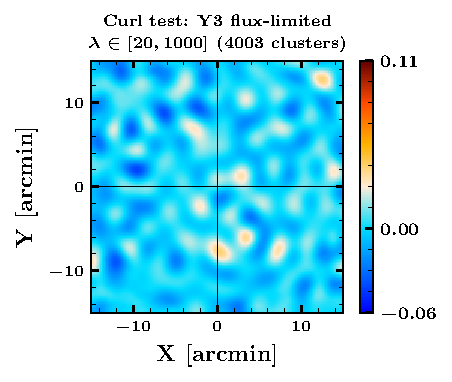
\includegraphics[width=\linewidth]{figs/kappa_model_MF_y3_v6_4_22_full_curl_test_JODY.pdf}
\caption{Stacked result of the curl test performed at the cluster locations by replacing the divergence operator in Eq. (\ref{eq_QE_kappa}) with a curl operator. %Both the tests are consistent with a null signal. 
We obtain a PTE value of 0.26, consistent with a null result.
%indicating that the null hypothesis of no-lensing is true.
%%The contours represent regions above $3.5\sigma$.
For the ease of visual comparison we adopt the same colour scale as in Fig. \ref{fig_QE_stacked_maps}.
}
\end{figure}
\subsection{Systematic error budget}\label{sec_sys_checks}

Now we consider possible sources of systematic error. %budget for the mass constraints reported in \S\ref{sec_results}. 
%assess the robustness of the constraints on the \ML scaling relation reported in \S\ref{sec_ML_scaling} against various systematic errors. 
%The sources of systematic uncertainty we consider include
 We estimate the bias due to each cluster's tSZ emission and residual foregrounds, the assumption of an underlying cluster profile, uncertainties in the DES RM mis-centering parameter $f_{\rm mis}$, approximations to the filter transfer function (Eq.~\ref{eq_filter_TF}), uncertainties in the beam measurements, and the assumption of a background cosmology.
Another source of systematic error is the uncertainties in the cluster redshifts estimated photometrically.
%But we ignore them in this work as \citetalias{raghunathan17a} demonstrated that the impact of photo$-z$ errors is negligible. 
However impact of photo$-z$ errors was estimated to be negligible by \citetalias{raghunathan17a}, and we ignore them here.
%Throughout this section we report the bias as the shift in the average lensing mass  of the DES RM \whichyear\ flux-limited sample clusters obtained using the \ML relation with the best-fit values to be reported in Fig. \ref{fig_massrichness_fitting}.

We rely on the \citetalias{sehgal10} simulations to estimate the level of residual-SZ/foreground bias in the RM \whichyear{} flux-limited sample.
In all the other cases we use the data and report the shift in the average lensing mass of the clusters in the RM \whichyear{} volume-limited sample obtained in \S\ref{sec_results}. %for the \whichyear\ flux-limited sample. % with our baseline analysis \mbox{(\sptpol{} tSZ-free $\times$ 150 GHz)}.
The combined systematic error budget is presented in Table~\ref{tab:sys}.
The systematic error calculated as a quadrature sum of the errors presented in Table~\ref{tab:sys} is much smaller than the statistical error in the measurements at a level of $0.15\sigma$. 
Using a direct sum, the combined error budget is $0.27\sigma$.
The dominant error comes from the uncertainty in the DES RM cluster centroids shifting the mean lensing mass by 2.8\%. 
%6.4\% for the full and volume-limited samples.


\subsubsection{Cluster tSZ signal and residual foregrounds}\label{subsec_tszbias}

\begin{figure}
\centering

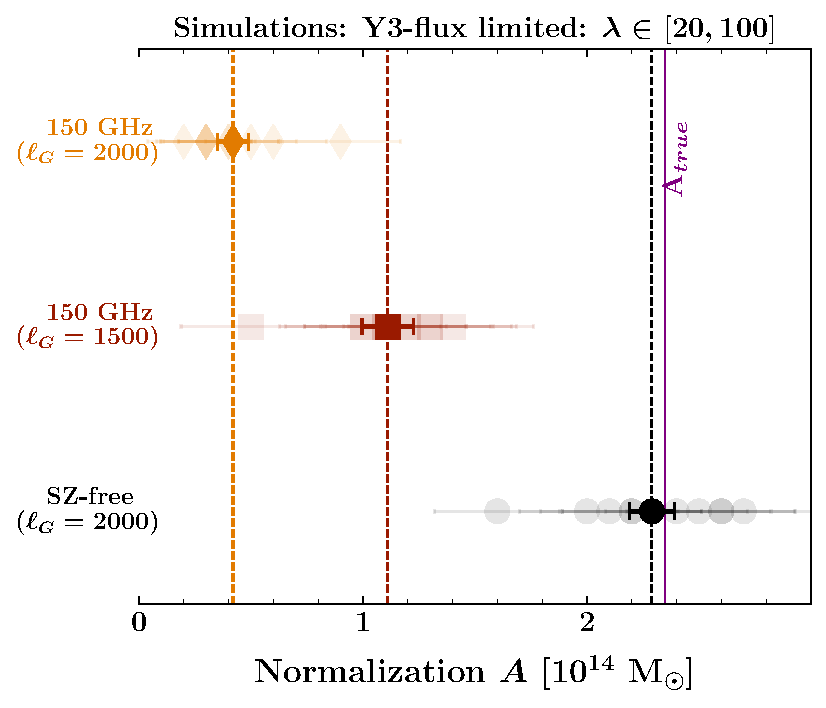
\includegraphics[width=0.45\textwidth, keepaspectratio]{figs/tsz_bias_checks_sehgal_sims.pdf}
%\caption{The recovered normalization parameter of the \ML relation for our fiducial analysis with $T^{\tszfreemapnotation}$ and $T^{150}$ in the two legs of the QE is shown in purple. The equivalent results with just the 150 GHz and different $\ell_{\rm G}$ = 1500 (2000) cutoff scales for the gradient estimation is shown in red? (orange) colors. }
\caption{ss}
\label{fig_QE_sehgal_sims}
\end{figure}

In this work we eliminate the bias due to SZ signal in the reconstructed lensing maps using  maps to estimate the background gradient of the CMB. 
%Since \sptpol{} has only two frequency channels, a simple tSZ cleaning operation will tend to modify other frequency dependent foregrounds and the resultant map is not an optimal foreground free CMB map for the lensing reconstruction. 
However, projecting just the tSZ signal out tends to modify other frequency-dependent foregrounds, and the resultant map is not an optimal foreground-free CMB map for the lensing reconstruction. 
This enhancement of foregrounds generally acts as an additional source of noise and tends to increase the variance of the reconstructed lensing maps. 
At the cluster locations, however, an increase in foreground emission due to galaxies inside the cluster can introduce undesired mode coupling between the estimated gradient map and the lensing map resulting in a biased lensing signal. 
Since massive clusters host more galaxies, we can expect the bias to increase with the cluster mass or equivalently richness. 
Here we quantify this bias using the \citetalias{sehgal10} foreground simulations.

To this end, we begin with the simulated skies described in \S\ref{sec_sims_funda}\pending{in previous chapter}, to which we then add simulated clusters, including the lensing signal (only the {\it 1-halo} term), thermal and kinetic SZ effects, and emission associated with the cluster (e.g. from member galaxies). %(like dusty galaxies). 
These simulations also include foregrounds uncorrelated with the clusters such as field radio galaxies.
%The foregrounds, unless specified otherwise, come from the \citetalias{sehgal10} simulations described below.
%Note that the foreground maps, whether associated with the cluster or not, are not lensed by the cluster in these simulations. 
The addition of foregrounds using \citetalias{sehgal10} simulations is described below. 
Note that the foreground maps, whether associated with the cluster or not, are not lensed by the cluster in these simulations. 
The number of simulated clusters and their redshifts and richnesses are derived from the  DES RM \whichyear{} flux-limited sample. 
The richnesses and redshifts are converted to cluster masses according to the \ML{} relation (Eq.~\ref{eq_ML}) with best-fit parameters from \citet{melchoir17}, $A_{\rm M17} = 2.35\ \times$ \munits, $\alpha_{\rm M17} = 1.12$, and $\beta_{M17} = 0.18$.  

For foregrounds, we extract half-arcminute resolution \boxsize\ cutouts of the 95 and 150 GHz \citetalias{sehgal10} simulations of the tSZ, kSZ, radio, and infrared galaxies around halos corresponding to the mock cluster sample. %the mass and redshift of the clusters in the DES RM \whichyear\ flux-limited sample. 
We scale the SZ power down from the \citetalias{sehgal10} simulations by a factor of 1.75 to match the \citet{george15} measurements.
%The \citetalias{sehgal10} simulations contain 16,000 halos above \mvir\ $\ge$ \munits\ and 175 halos above \mvir\ $\ge 5 $ \munits\ at redshifts $z \ge 0.25$.
These foreground cutouts are added to our mock galaxy cluster lensed CMB datasets. %instead of the Gaussian realizations of the extragalactic foregrounds described earlier. 
The maps are then processed in the same way as explained in \S\ref{sec_method_QE} to extract the SZ cleaned map and passed into the QE. 

%Like discussed in \S\ref{sec_pipeline_validation}, we pick clusters in the richness range $\lambda \in [20, 100]$ from the DES RM \whichyear\ flux-limited sample for this test. Like in \S\ref{sec_pipeline_validation}, we use the \ML{} relation with best-fit parameters from DES \citet{melchoir17} to convert richness estimates into masses.

We present the results in Fig. \ref{fig_QE_sehgal_sims}.
%The true normalization \mbox{$A_{true} = 2.35\ \times$ \munits} adopted from \citet{melchoir17} is shown as the purple solid line.
The true normalization is shown as the purple solid line.
In the figure, the light shaded data points are the result for a single simulation run ($\sim$ 4000 clusters) and the darker data points are the results for $10\times$ the sample size. 
%As explained in \S\ref{sec_pipeline_validation}, in 
%For our baseline analysis with  maps for the gradient estimation and $\ell_{\rm G} = 2000$, the recovered normalization is $\la0.5\sigma$ from the true value.
We obtain \mbox{$A = 2.30 \pm 0.09\ \times$ \munits} (black circle) implying no significant residual foreground bias in the lensing measurements.
%This result also asserts that the lensing pipeline is unbiased.
This result also provides evidence that the lensing pipeline is unbiased.

{\it Comparison to standard QE:} We also use the \citetalias{sehgal10} simulations to compare the modified QE to the standard case using the 150 GHz map for the background CMB gradient estimation.
In the standard case, the correlations introduced between the two maps by the foregrounds, the tSZ signal in particular, can be alleviated by lowering the LPF threshold $\ell_{\rm G}$ for the gradient map as in Eq. (\ref{eq_QE_filters}). 
As described in \S\ref{sec_method_QE}, the choice of $\ell_{\rm G}$ is a trade-off between the level of foreground bias and the lensing \snr{}. 
%Here we adopt $\ell_{\rm G} = 2000$ and $\ell_{\rm G} = 1500$.
%On the other hand, the results for the standard QE case are heavily biased: red squares (orange diamonds) for $\ell_{\rm G} = 1500$ ($\ell_{\rm G} = 2000$).
Here we adopt $\ell_{\rm G} = 2000$ and $\ell_{\rm G} = 1500$ and note that the results are heavily biased in both cases: red squares (orange diamonds) for $\ell_{\rm G} = 1500$ ($\ell_{\rm G} = 2000$).
The level of bias is higher when $\ell_{\rm G}$ is set to 2000 compared to 1500, as expected.
This bias is predominantly due to the tSZ signal and can be reduced by removing massive clusters from the analysis as in \citetalias{baxter18}. 
For comparison, when we apply a richness cut of $\lambda \in [20, 40]$ the lensing bias is reduced from 82\% to 65\% for $\ell_{\rm G} = 2000$ and 52\% to 35\% for $\ell_{\rm G} = 1500$. 
This cut removes $\sim$500 massive clusters from the analysis.
This result can be compared to the conservative tSZ-bias of 11\% set by \citetalias{baxter18} with $\ell_{\rm G} = 1500$ for the same richness range $\lambda \in [20, 40]$.
%They obtain a lower bias value as the high-$\ell$ modes in the SPT-SZ maps are down-weighted compared to the \sptpol{} maps which have a $4\times$ lower noise.
\citetalias{baxter18} obtained a lower bias value as the high-$\ell$ modes in the SPT-SZ maps are down-weighted due to $4\times$ higher noise.
%This also suggests that we cannot handle the tSZ bias by simply removing clusters above a certain richness, for example $\lambda \ga 40$, for low-noise CMB datasets.

Finally, a subtle point from the figure is that the mass constraints obtained using the 150 GHz map for gradient estimation
(orange diamonds) are better ($\sim$ 14\%) than those obtained using the tSZ-free map for gradient estimation (black circles) despite adopting $\ell_{\rm G} = 2000$ in both cases.
%This hit in the \snr{} arises because the \sptpol{} \tszfreemapnotation{} map is noisier than the 150 GHz.
 \subsubsection{Cluster profile}\label{subsec_clusprofile}
%In our fiducial analysis we obtain lensing mass measurements by assuming that the underlying halo profile of the clusters obey the NFW dark matter model. 
%However the true profile of galaxy clusters could be different from a smooth NFW model and deviations from the NFW profile have been observed in earlier works \citep{diemer14}. 
%Furthermore, as argued by \citet{child18}, Einasto model is a better fit to `stacked' halo profiles compared to the NFW.
In our fiducial analysis, we assume that the underlying halo profile of the clusters follows the NFW dark matter model. 
However,halos in real clusters %the true profile of galaxy clusters may not follow the NFW model and indeed 
deviations from the NFW profile have been observed \citep[e.g.,][]{diemer14}, and 
\citet{child18} argued that the Einasto model is a better fit than NFW to stacked halo profiles.
%In this section, we estimate the bias in the lensing mass due to the assumption of the NFW profile by using an Einasto profile \citep{einasto89} to model the lensing convergence during the fitting process.
%But considering the efficacy of comparing our results to other similar works in the literature, we use NFW for our baseline analysis.

%In this section, we validate the assumption of NFW profile using an Einasto profile \citep{einasto89} to model the lensing convergence $\kappa^{1h}$ during the fitting process.
In this section, we estimate the magnitude of a possible bias due to the assumption of the incorrect mass profile by using an Einasto profile \citep{einasto89} to model the lensing convergence $\kappa^{1h}$.
% during the fitting process.
The lensing QE and subsequently the reconstructed convergence maps remain unchanged.
The Einasto profile is defined as
\begin{eqnarray}
\rho(r)_{_{\rm Ein}} & = &  \rho_{_{0}}\ \mbox{exp}\left( - \frac{2}{\alpha} \left[\left(\frac{r}{R_{\rm s}} \right)^{\alpha} - 1\right]\right),
%\rho(r)_{_{\rm Ein}} & = &  \delta_{c}\rho_{mean}^{z}\ e^{\left( - \frac{2}{\alpha} \left[\left(\frac{r}{R_{\rm s}} \right)^{\alpha} - 1\right]\right)}
\label{eq_einasto_density}
\end{eqnarray}\\
%where $R_{\rm s}$ is the scale radius, $\delta_{c}$ is the characteristic over-density, $\rho_{mean}^{z}$ is the mean-density of the Universe at the cluster redshift, and $\alpha = 0.18$ is the shape parameter \citep{ludlow13}. 
where $\alpha = 0.18$ is the shape parameter \citep{ludlow13}. 
As in the NFW analysis, the concentration $c_{200}$ as a function of mass and cluster redshift is obtained using the \citet{duffy08} relation.
We use the general framework for spherically symmetric halos defined in \citetalias{raghunathan17a} and simply plug the above density profile into Eq. (2.9) of \citetalias{raghunathan17a} to obtain the Einasto convergence \kappaonehalo$^{,\rm Ein}$ profiles. The \kappatwohalo\ term remains the same. For the Einasto case we see a negligible shift of $0.01\sigma$ compared to our fiducial result.
%The shift in the lensing mass of the DES RM clusters is negligible. 
\subsubsection{Uncertainties in filter transfer function and beam}\label{subsec_TF}
As described in \S\ref{sec_data}, the \sptpol{} map-making process is lossy, with noisy modes along the scan direction filtered out. 
The ideal, if computationally expensive, approach to handle the filtering would be an end-to-end simulation from the TOD to the lensing reconstruction. 
In this work, we take a computationally much cheaper approach and approximate the filtering by the phenomenological fit to the filter transfer function in Fourier space given by Eq. (\ref{eq_filter_TF}). 
The major uncertainty is in the position of the high-pass filter (HPF) in the scan direction: this filters modes more strongly than the isotropic HPF, and the LPF is at angular scales that do not matter to the reconstruction. 
The estimated position for this HPF is $\ell_x = 300 \pm 20$. 
%Thus we evaluate the recovered mass for an assumed $\ell_x=$280 and 320 in Eq. \ref{eq_filter_TF}.
%The model, however, remains fixed at $\ell_x = 300$ in both the cases.
We also recompute the models for an assumed $\ell_x = 280$ and 320 to evaluate the shifts in the lensing masses.
%Ideally, one can expect the lensing masses to shift low and high for the two cases compared to our fiducial result.
We note no significant effect (masses shift by roughly $\pm 0.02\sigma$), indicating that the uncertainty in the simplified filtering treatment causes negligible changes to our results.
%%\pending{Pending: SR: Will it be better to test this using simulations instead?.}

Similarly, we also check the effect of errors in the telescope beam modeling \beambl{} that were derived using Venus observations (see \S\ref{sec_sptpol}). 
We find that the effect due to beam uncertainties in the final result is also negligible. 
The shift in the lensing mass is%$\la 0.01\sigma$ when we modify \beambl{} $\rightarrow$ \beambl{} $+\ 2\sigma$.
%For the Einasto profile we obtain a lensing mass of \sysbiaseinastoresult\ for the stacked sample. While the mass is slightly higher, it is only $0.2\sigma$ off from our fiducial result implying that the bias due to the assumption of the NFW profile is negligible. 
\subsubsection{Underlying cosmology}\label{subsec_others}
%In this section we estimate the effect of the assumption of a background cosmology on the lensing measurements. 
The systematic error arising due to the assumption of a background cosmology is quantified here.
As described in earlier sections, in our fiducial analysis we use the \lcdm\ cosmology obtained using the \planck\ 2015 datasets \citep{planck15-13}. 
%Here we repeat the analysis by slightly changing the background cosmology. 
%Specifically, we generate new lensed CMB power spectra using \texttt{CAMB} by adding $1\sigma$ errors to the \planck\ 2015 cosmological parameters and similarly by altering the beam by \beambl $+\ 2\sigma$. 
Here we repeat the analysis by modifying the lensed CMB power spectra $C_{\ell}$ to include the $1\sigma$ errors to the \planck\ 2015 cosmological parameters.
Modifying the background cosmology alters the weights of Eq. (\ref{eq_QE_filters}) in the lensing estimator and also the model convergence profiles \kappaonehalomz\ and \kappatwohalomz. 
However, the effect due to background cosmology in the inferred lensing mass is negligible with a shift in the lensing mass %$\la 0.03\sigma$.
%\subsection{Offsets in the stacked convergence map}\label{subsec_offsets}
%\section{NFW profile}

  \section{Results and Discussion}\label{sec_results}

The main results of this work are the lensing-derived cluster mass constraints for the DES RM \whichyear\ cluster samples using \sptpol{} tSZ-free $\times$ 150 GHz temperature maps.
%using three different combination of the \sptpol{} and \planck{} temperature maps: (A) \sptpol{} tSZ-free $\times$ 150 GHz maps (baseline); (B) \lgmca $\times$ \sptpol 150 GHz maps; and (C) baseline $+$ \sptpol{} tSZ-free $\times$ tSZ-free maps for clusters with $\lambda \ga 40$.
Below, we first present the lensing mass estimates in \S\ref{sec_temp_results} and use the lensing measurements from the DES \whichyear{} volume-limited sample to independently calibrate the \ML{} relation of the cluster sample in %\S\ref{sec_ML_scaling}. 
\subsection{Stacked mass measurements}
\label{sec_temp_results}
In Fig. \ref{fig_QE_stacked_maps}, we present the results of our stacked lensing measurements. 
The left (right) panel correspond to the convergence maps stacked at the location of clusters in the DES \whichyear\ flux(volume)-limited sample.
The variance in the flux-limited sample is lower than the volume-limited sample because the flux-limited sample has twice as many objects. 
An estimate of the mean-field has been subtracted from the maps.
We reject the null hypothesis of no lensing with a significance of \howmanysigmaforfullsample\ for the flux-limited sample of \howmanyclustersinfullsample\ clusters. 
The obtained \snr{} is consistent with our expectations from the simulations shown as lighter black circles in %Fig. \ref{fig_QE_sehgal_sims}.
For the smaller volume-limited sample, the no-lensing hypothesis is ruled out at  \howmanysigmaforcosmosample.
The radially binned convergence profiles that are used to estimate the cluster masses are shown in Fig. \ref{fig_QE_stacked_maps_radprf} along with the best-fit model curves. 
\begin{figure}
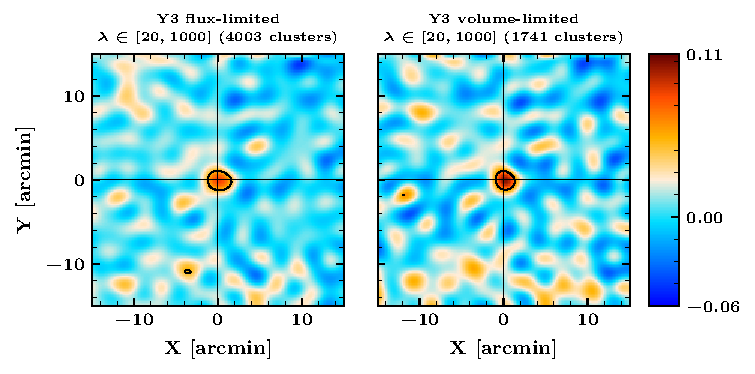
\includegraphics[width=\linewidth]{figs/kappa_model_MF_y3_v6_4_22_full_vl_JODY.pdf}
\caption{It shows}
\label{fig:fig_QE_stacked_maps}
\end{figure}

\begin{figure}
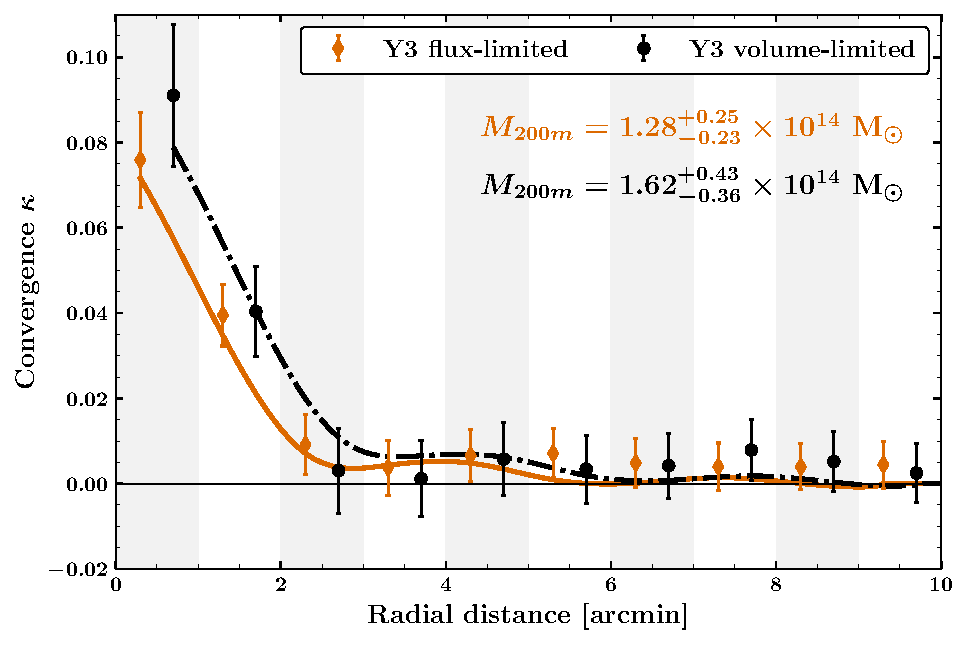
\includegraphics[width=\linewidth]{figs/kappa_model_MF_y3_v6_4_22_full_vl_radprf_JODY.pdf}
\caption{It shows}
\label{fig:fig_QE_stacked_maps}
\end{figure}

The ringing pattern is because of the sharp filtering of modes above the \sptpol{} beam scale. 
The error bars plotted are the square root of the diagonal entries of the covariance matrix estimated using %Eq. (\ref{eq_JK_cov}). 
%As explained in \S\ref{sec_nfw_model_fitting}, all the mass estimates are derived by fitting a NFW profile along with the contribution from the {\it 2-halo} term to the measured radially binned profile. 
The recovered lensing masses for the stacked flux and volume-limited samples are %\mbox{\mvir = \fitmassforfullsamplewitherrors\ \times \munits} and \mbox{\fitmassforvlsamplewitherrors\ \times \munits} respectively. 
According to expectations, the lensing masses shift up by 0.3$\sigma$ when the {\it 2-halo} term is excluded.


A higher mean mass is expected for the volume-limited sample. 
At redshifts above $z\sim 0.6$, galaxies at the luminosity threshold adopted by RM become too faint to be detected in the DES data. 
Consequently, the richness of the clusters is extrapolated from the subset of galaxies that are sufficiently bright to be detected. 
This extrapolation introduces additional noise in the richness estimates.
The increased scatter leads to more low-mass systems scattering up to apparently rich systems, thereby lowering the mean mass of the selected halos. 
For this reason, we restrict our analysis to the volume-limited sample in the subsequent sections. 
\subsection{Mass-richness \ML{} scaling relation calibration}\label{sec_ML_scaling}

We now apply the lensing mass measurements from \S\ref{sec_temp_results} to constrain the relationship between a cluster's mass, $M$, and optical richness, $\lambda$, in the DES RM \whichyear{} volume-limited sample. 
We limit the analysis to just the volume-limited sample since the flux-limited sample has selection bias as explained above in \S\ref{sec_temp_results}.
%Due to its higher S/N, we use the QE  with a tSZ-free gradient map; we do not combine the two estimators due to the complexity in combining the different bases of the MLE and QE. 
Following earlier weak-lensing analyses of RM clusters \citep{simet18, melchoir17, mcclintock18}, we use a power-law scaling relation for cluster mass, $M$, as a function of richness, $\lambda$, and redshift, $z$,
\begin{eqnarray}
M = A \left(\frac{\lambda}{40}\right)^{\alpha} \left(\frac{1+z}{1+0.35}\right)^{\beta},
\label{eq_ML}
 \end{eqnarray}
 where $A$ is a normalization parameter, and the exponents $\alpha$ and $\beta$ are richness and redshift evolution parameters respectively. 
The pivot points for the richness and redshift evolution were set based on DES weak-lensing measurements of \citetalias{mcclintock18}.
%Given the total\snr{}is of order eight for the flux-limited sample, we do not subdivide the stacks into different richness or redshift bins. 
The model for the stacked mass is 
\begin{equation}
M(A, \alpha, \beta) \equiv M = \frac{\sum_j w_j M(\lambda_{j}, z_{j})}{\sum_j w_j}, 
\label{eq_model_ML}
\end{equation}
where the sum runs over the number of clusters in the sample and the weight $w$ for each cluster is given in Eq. (\ref{eq_cluster_weight}).

We do not split the stacks into different richness or redshift bins.
As a result, the data's sensitivity to the two evolution parameters is minimal and we apply informative priors to both.
We perform a Markov chain Monte Carlo (MCMC) analysis %with 100 walkers and 750 steps each 
using the publicly available \emph{emcee} \citep{mackey13} code to sample the likelihood space.
%The first 100 steps from all walkers were discarded as the burn-in phase.
\begin{figure}
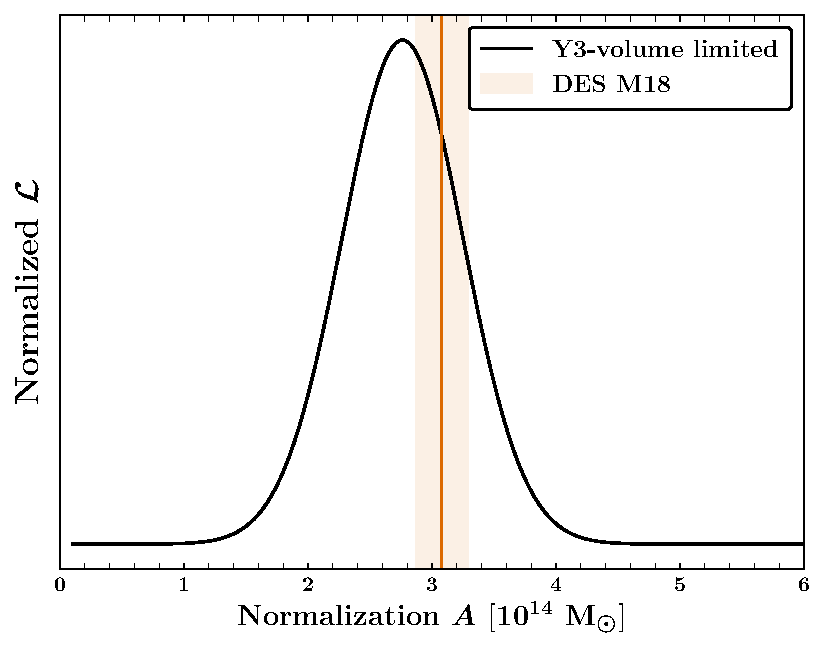
\includegraphics[width=\linewidth]{figs/M_rich_fitting_y3_v6_4_22_full_vl_JODY.pdf}
\caption{It shows}
\end{figure}
subsection{Comparison to literature}\label{subsec_lit_comparison}
We now compare our results to similar works from the literature performed with the RM cluster catalogs from the SDSS and DES experiments. 
Since the richness estimated for a given cluster from surveys A and B can vary slightly depending on the adopted data reduction and analysis choices, we include a a small correction factor $\epsilon_{\rm A{\text -}B}$ when comparing results from two surveys.
We compute the ratio $\lambda_{\rm A}/\lambda_{\rm B}$ for the overlapping clusters in the two surveys and simply set $\epsilon_{\rm A{\text -}B}$ to the median value of the ratios.
We find the richness estimates in DES Year-3 and Year-1 to be consistent with $\epsilon_{\rm Y3{\text -}Y1} = 1$. 
For the rest, we set: $\epsilon_{\rm Y3{\text -}SV} = 1.08$ and $\epsilon_{\rm Y3{\text -}SDSS} = 0.93$ \citepalias{mcclintock18}.
The comparison after including this correction factor is presented in Fig. \ref{fig_lit_comparison}, which is similar to Fig. 15 in \citetalias{mcclintock18}. 
%Specifically, we show the difference in \mvir masses obtained from different works for a cluster with richness $\lambda = 40$ at redshift $z=0.35$, the pivot points in Eq. (\ref{eq_ML}).
The figure is normalized using the $1\sigma$ error from the current work with the \whichyear{} volume-limited DES RM catalog sample.

%In the figure, \citet{simet18} and \citet{geach17} works use the SDSS RM catalog sample containing roughly 26,000 clusters while the other use DES RM catalogs.
Each analysis uses a different cluster sample and lensing data.
\citet{simet18} and \citet{geach17} use the SDSS RM catalog sample containing roughly 26,000 clusters. % while the other use DES RM catalogs.
%Among the DES works, 
\citet{melchoir17} use the full catalog from the DES science verification data while \citetalias{baxter18} and \citetalias{mcclintock18} perform the analysis using the DES Year-1 volume-limited sample.
The works by \citet{geach17} and \citetalias{baxter18} use the CMB-cluster lensing technique (filled points) with \planck{} and {\sc SPT-SZ} CMB temperature maps.
All the others use galaxy weak-lensing measurements and are represented as open points. As evident from the figure, our results are consistent with other similar works in the literature.

\begin{figure}
\centering
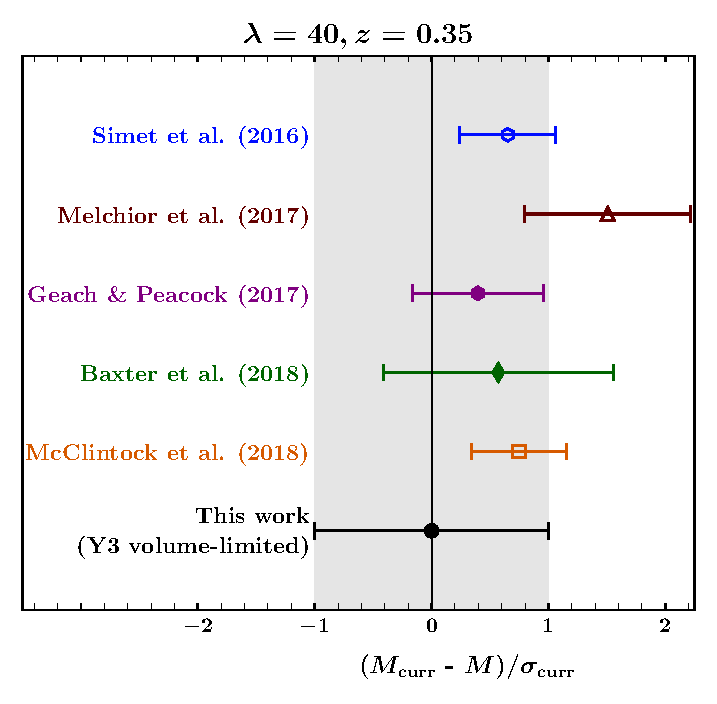
\includegraphics{figs/lit_comparisons_JODY.pdf}
\caption{ss}
\label{fig_lit_comparison}
\end{figure}